\documentclass{article}
\usepackage[utf8]{inputenc}
\usepackage[french]{babel}
\usepackage[left=2.5cm,right=2.5cm,top=3cm,bottom=3cm]{geometry}
\usepackage{hyperref}
\usepackage{graphicx}
\usepackage{float}
\usepackage{indentfirst}
\usepackage{cite}

\setlength\tabcolsep{10pt}


\title{Projet de Conception~: Calcul Parallèle et évaluation de performance}
\author{Xavier Dussert-Vidalet, Marc-Antoine Fernandes et Louis Sugy}
\date{January 2019}

\begin{document}

\maketitle

\setlength{\parskip}{1.5mm}

\tableofcontents
\newpage

\setlength{\parskip}{3mm}

\section{Introduction}
\subsection{Mise en contexte}

Ce projet consiste à optimiser un simulateur d'évolution grâce au calcul parallèle et aux accélérateurs graphiques présents sur nos machines. Cet algorithme se porte très bien à la parallélisation, car il est composé d'une succession d'étapes identiques pour chaque "cellule". Ces cellules sont similaires, nombreuses et quasiment indépendantes. Ainsi les étapes de calculs peuvent être effectuées de manière isolée, jusqu'au moment de la synchronisation. Cette synchronisation est effectuée à la fin de chaque étape, et permet de sélectionner les meilleurs cellules pour les générations suivantes.

Nous avions le choix entre utiliser OpenMP, OpenACC ou CUDA pour la parallélisation. Nous avons décidé d'utiliser CUDA pour nous familiariser avec ce langage et cette manière de programmer. Nous avons rencontré des difficultés à l'exécution sur certaines de nos machines mais nous sommes parvenus à le faire tourner sur un de nos ordinateurs.

Dans ce document nous présentons les différentes optimisations que nous avons faites ainsi que leur comparaison au niveau des performances. Il faut tenir compte du fait que nous n'avons pas eu le temps de faire l'intégralité des optimisations que nous voulions faire, ce qui donne des allers-retours entre le GPU et le CPU. Ces allers-retours ralentissent le programme avec des charges I/O supplémentaires.


\subsection{Démarche}

Pour aborder ce projet, nous avons commencé par prendre connaissance du code, éliminer les parties inutiles ou redondantes et faire un peu de refactoring. Puis nous avons fait un première évaluation de performance pour identifier les parties du code les plus coûteuses. Pour cela, nous avons utilisé l'outil \texttt{callgrind} de \texttt{valgrind}, qui permet d'obtenir l'arbre d'appel des fonctions avec les pourcentages de temps CPU utilisés (temps propre et temps incluant les appels de fonctions). La figure \ref{fig:callgrind} montre un extrait des résultats.

\begin{figure}[H]
\centering
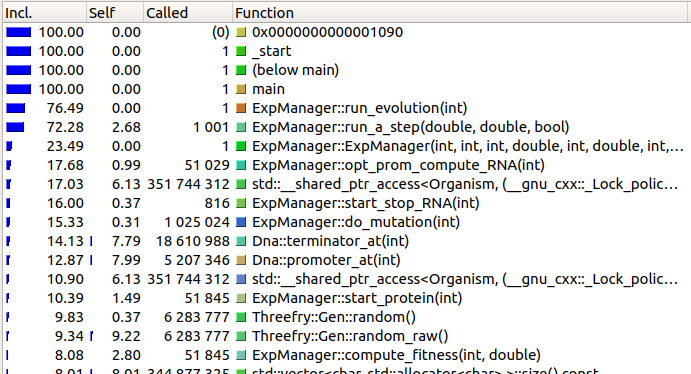
\includegraphics[width=0.8\textwidth]{callgrind.png}
\caption{Fonctions les plus coûteuses identifiées par \texttt{callgrind}}
\label{fig:callgrind}
\end{figure}

Cette évaluation nous a permis de cerner quelques points critiques de l'application, par exemple on remarque que la recherche de promoteurs et terminateurs prend 20\% du temps (voire plus si on ne considère pas tous les coûts d'initialisation). C'est donc une partie intéressante à paralléliser.

\section{Étape de sélection en CUDA}

Le principe de l'étape de sélection est de choisir, pour chaque élément d'une grille d'individus, lequel de lui ou d'un de ses voisins sera sélectionné pour les étapes suivantes, avec une probabilité proportionnelle à sa fitness.

\subsection{Implémentation}

Cet algorithme correspond à un pattern de calcul parallèle appelé \textit{stencil}. Nous avons choisi de passer en entrée du kernel un tableau de fitness des individus, et de rendre en sortie un tableau du voisin choisi pour la prochaine génération. Dans notre implémentation du stencil, nous avons choisi que chaque thread chargerait une valeur en mémoire partagée, et les threads correspondant à l'intérieur des blocs calculeraient chacun le prochain voisin pour un individu.

\subsection{Évaluation de performances}

Pour évaluer la performance de la version GPU de la sélection, nous avons comparé le temps passé à calculer la sélection sur GPU et sur CPU. Pour la version GPU, nous avons calculé le temps total en comptant les transferts de données, et le temps passé sur le calcul seul. Dans un premier temps, nous avons eu des résultats très décevants car le calcul était aussi long que sur CPU (et avec le transfert, l'opération était globalement plus lente). Notre erreur était d'utiliser un \texttt{new} et \texttt{delete}, ce qui en CUDA fait une allocation dans la mémoire globale et non celle du thread. Une fois ce problème résolu, nous avons obtenu des performances très satisfaisantes, comme le montre la comparaison présentée dans le tableau en figure \ref{fig:selection_comp}.

\begin{figure}[H]
\centering
\begin{tabular}{|c|c|c|}
    \hline
    CPU & GPU (transferts inclus) & GPU (calcul) \\
    \hline
    796.8 & 153.2 & 51.7 \\
    \hline
\end{tabular}
\caption{Temps moyen en microsecondes de la sélection}
\label{fig:selection_comp}
\end{figure}

Le facteur de performance 15 du calcul est inférieur à l'espérance théorique de 1024, puisqu'il y a le temps de lancement du calcul sur GPU, des latences liées aux lectures et écritures dans la mémoire globale du GPU, et une certaine divergence des chemins~: \textit{Nvidia Visual Profiler} rapporte que $56.7\%$ des threads sont actifs en moyenne dans chaque warp. Cette divergence peut s'expliquer d'une part par la bordure du stencil, d'autre part par les boucles \texttt{while} dans le code de la fonction \verb|roulette_random|.

\section{Recherche de promoteurs et terminateurs en CUDA}

Une étape très coûteuse en temps est celle de recherche des promoteurs et terminateurs dans la séquence d'ADN des individus. Dans le code CPU fourni, celle-ci était optimisée pour ne rechercher qu'autour des mutations dans la séquence lors des générations ultérieures à la première. Cette approche n'est pas adaptée à la version GPU car elle dynamique et implique de lancer de nombreux kernels sur de petits segments d'ADN, alors qu'il est plus efficace sur GPU de faire un seul gros transfert de données puis des recherches à de nombreux endroits en parallèle.

\subsection{Implémentation}

Pour implémenter la recherche, nous avons écrit deux kernels au fonctionnement similaire (un pour les promoteurs et un pour les terminateurs). Chaque bloc reçoit un segment d'ADN et charge celui-ci en mémoire partagée (en effet cela permet de diviser le nombre d'accès à la mémoire globale par la taille des promoteurs / terminateurs). Ensuite, une partie des threads du bloc regarde si un promoteur ou terminateur commence à cette position en bouclant à partir de celle-ci. Pour faire remonter les résultats, nous utilisons une pile de positions. Celle-ci est remplie à l'aide d'un index de fin incrémenté atomiquement comme suit~:

\begin{verbatim}
uint pos_to_write = atomicAdd(&pos_prom_counter[indiv_id], 1);
promoters[indiv_id * genome_size + pos_to_write] = i;
\end{verbatim}

Le code CPU se charge de récupérer ces positions, les trier et les ajouter dans les structures de données appropriées. L'opération \verb|compute_RNA| est effectuée sur CPU.

\subsection{Évaluation de performances}

Pour l'évaluation de cette méthode, nous avons comparé le temps d'exécution de la recherche sur CPU et GPU, et pour GPU nous avons comparé l'utilisation de plusieurs tailles de blocs différentes. Ces résultats sont présentés dans la figure \ref{fig:search_comp}.

\begin{figure}[H]
\centering
\begin{tabular}{|c|c|c|c|c|}
    \hline
    CPU & GPU (128) & GPU (256) & GPU (512)  & GPU (1024) \\
    \hline
    92104 & 16011 & 15862 & 12025 & 8860 \\
    \hline
\end{tabular}
\caption{Temps moyen en microsecondes de la recherche, par taille de bloc pour le GPU}
\label{fig:search_comp}
\end{figure}

Ces résultats montrent que, pour le même algorithme, la version GPU est jusqu'à 10 fois plus efficace que la version CPU non optimisée (même en comptant les transferts de données). L'évaluation montre également que le choix de taille de bloc de 1024 est le plus performant ici. En revanche, en toute honnêteté intellectuelle il se doit de comparer la version GPU (avec \verb|compute_RNA| sur CPU) à la version CPU optimisée \verb|opt_prom_compute_RNA| qui ne recherche qu'autour des nouvelles mutations. La figure \ref{fig:honest_comp} montre les résultats de cette comparaison. La version GPU ne parvient donc pas à faire mieux que l'optimisation sur CPU. En revanche, on peut penser qu'avec plus de mutations, le coût CPU deviendrait plus élevé alors que le coût GPU ne changerait pas.

\begin{figure}[H]
\centering
\begin{tabular}{|c|c|}
    \hline
    CPU avec optimisation & GPU (taille de bloc~: 1024) \\
    \hline
    2218 & 11069 \\
    \hline
\end{tabular}
\caption{Temps moyen en microsecondes de la recherche avec la version CPU optimisée, et la version GPU avec \texttt{compute\_RNA} sur CPU}
\label{fig:honest_comp}
\end{figure}

\section{Conclusion}

Ce projet nous a mis dans une situation réelle d'optimisation d'un logiciel existant à l'aide de GPU. Même si ces optimisations requièrent un certain temps de mise en place et de refactoring du code, nous avons trouvé le résultat plus simple et maintenable que ceux à quoi nous nous attendions, et pour des performances assez impressionnantes (des facteurs 10 ou 15). Le code est plus compliqué à déboguer que du code séquentiel (on ne peut pas simplement mettre des points d'arrêts, retracer l'exécution, etc) et certaines spécificités de la plateforme ont pu nous bloquer, mais à force de pratique nous avons mieux pris en main ce paradigme de programmation.

\end{document}
